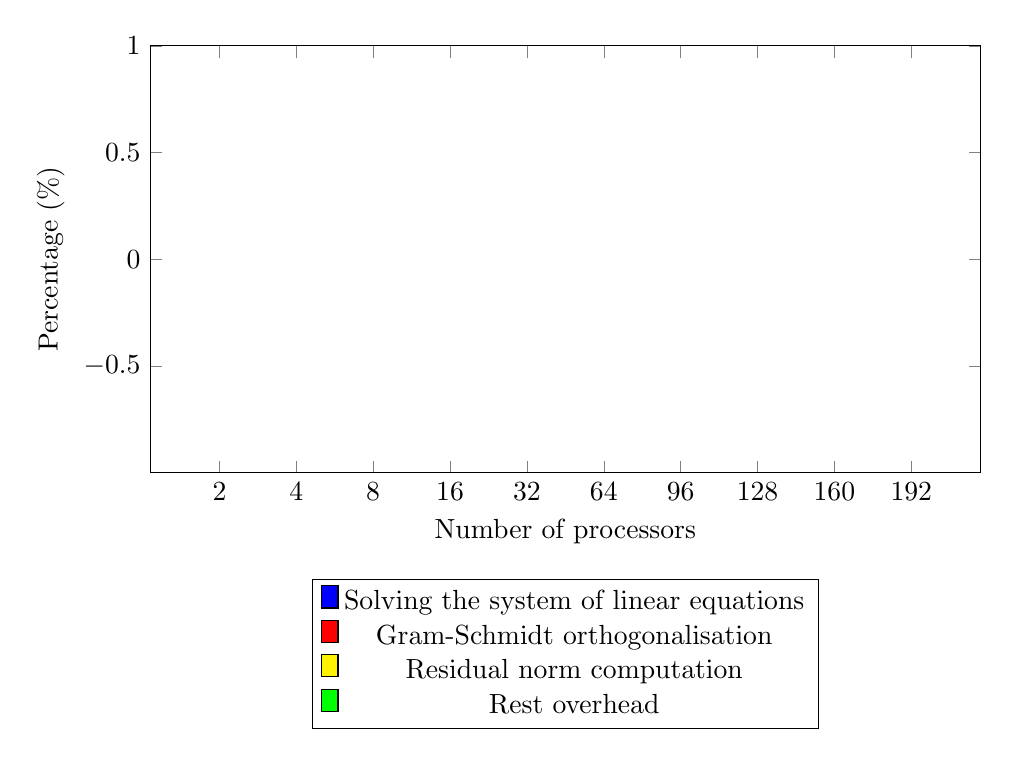
\begin{tikzpicture}
 \begin{axis}[
  ybar stacked,
  height=7cm,
  width=\textwidth,
  xlabel=Number of processors,
  symbolic x coords={2, 4, 8, 16, 32, 64, 96, 128, 160, 192},
  legend style={
   at={(0.5, -0.25)},
   anchor=north
  },
  ylabel={Percentage (\%)}]
  \addplot[ybar, fill=blue] plot coordinates {
   (2, 0)
   (4, 0)
   (8, 0)
   (16, 0)
   (32, 0)
   (64, 0)
   (96, 0)
   (128, 0)
   (160, 0)
   (192, 0)};
  \addplot[ybar, fill=red] plot coordinates {
   (2, 0)
   (4, 0)
   (8, 0)
   (16, 0)
   (32, 0)
   (64, 0)
   (96, 0)
   (128, 0)
   (160, 0)
   (192, 0)};
  \addplot[ybar, fill=yellow] plot coordinates {
   (2, 0)
   (4, 0)
   (8, 0)
   (16, 0)
   (32, 0)
   (64, 0)
   (96, 0)
   (128, 0)
   (160, 0)
   (192, 0)};
  \addplot[ybar, fill=green] plot coordinates {
   (2, 0)
   (4, 0)
   (8, 0)
   (16, 0)
   (32, 0)
   (64, 0)
   (96, 0)
   (128, 0)
   (160, 0)
   (192, 0)};
  \legend{
   Solving the system of linear equations,
   Gram-Schmidt orthogonalisation,
   Residual norm computation,
   Rest overhead}
 \end{axis}
\end{tikzpicture}
